% Plot Tiefpass
% Minimalistisch (sketch-like for beamer presentation)
% Amplitudengang
% plots with same width for vertical alignment:
%   plot_tiefpass_mini_ampli_lin_samesize.tex
%   plot_tiefpass_mini_phase_lin_samesize.tex
%   plot_hochpass_mini_ampli_lin_samesize.tex
%   plot_hochpass_mini_phase_lin_samesize.tex
% TODO: Alignment via invisible boundbox
\def\ttau{0.01}%                % Zeitkonstante tau = 0.01 s
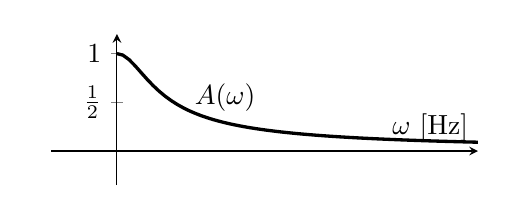
\begin{tikzpicture}%
    % invisible boundbox
    \draw[draw=none](-0.3,-0.125) rectangle (+5.5,+2); % bbox % set draw=black (debug) or draw=none (final)
    \begin{axis}[%
        xlabel={$\omega\ [\mathrm{Hz}]$},
        xmin=-200, xmax=1100,       % alignment solution with x-axis (bigger than y-labels):
        domain=0:1100, 
        ymin=-0.35, ymax=1.2,
        samples=61,
        axis x line=center,
        axis y line=center,
        width=7cm,
        height=3.5cm,
        ytick={0,0.5,1},
        yticklabels={$0$,$\frac{1}{2}$,$1$}, 
        xtick=\empty,
    ]   % A(omega) = 1/(1+(omega*tau)^2)^0.5
        \addplot[mark=none,very thick,]{1/(1+(x*\ttau)^2)^0.5}  node[pos=0.3,anchor=south] {$A(\omega)$};%  plot + plotlabel
    \end{axis}%
\end{tikzpicture}%